\documentclass[12pt, a4paper]{article}


% A pretty common set of packages
\usepackage[margin=2.5cm]{geometry}
\usepackage[T1]{fontenc}
\usepackage{graphicx}
\usepackage{amssymb}
\usepackage{amsmath}
\usepackage{bm}
\usepackage{color}
\usepackage{float}
\usepackage{bm}
\usepackage{physics}
\usepackage{subcaption}

\DeclareRobustCommand{\uvec}[1]{{%
  \ifcsname uvec#1\endcsname
     \csname uvec#1\endcsname
   \else
    \bm{\hat{\mathbf{#1}}}%
   \fi
}}
\newcommand{\olsi}[1]{\,\overline{\!{#1}}} % overline short italic

\usepackage[colorlinks=true, 
    linkcolor=blue,          % color of internal links
    citecolor=blue,        % color of links to bibliography
    filecolor=blue,      % color of file links
    urlcolor=blue]{hyperref}

\title{[16-833] Homework 4 : Written Report}
\author{Bharath Somayajula}
\date{\today}

\begin{document}

\maketitle

\tableofcontents

\section{Iterative Closest Point}
\subsection{Projective Data Association}
\subsubsection{Conditions}
For a source point to have a valid correspondence in target vertex map, it's projected coordinates must fall within the bounds of the vertex map and have a positive depth. Therefore, assuming that the u, v coordinates are rounded to integers and are zero-indexed, we get:
\[0 \leq  u < W\]
\[0 \leq  v < H\]
\[d > 0\]

\subsubsection{Distance Filtering}
Distance filtering is needed for a few reasons:
\begin{enumerate}
  \item We assume that change in pose is small between consecutive measurements. This implies that change in vertex map between consecutive frames is also small. So it makes sense to apply a distance thresholds
  \item Vertex map is constructed from depth map and depth measurements can be corrupted for several reasons such as noise, wildly inaccurate measurements due to surface properties of materials whose depth is being measured or in practical settings due to objects entering the scene between frames. Therefore, applying distance threshold is a reasonable way to overcome these issues.
\end{enumerate}
\subsection{Linearization}
The expression $(\delta R)p_i^{'} + \delta t$ needs to be simplified first.
\[(\delta R)p_i^{'} + \delta t = \begin{bmatrix}
  1 & -\gamma & \beta\\
  \gamma & 1 & -\alpha\\
  -\beta & \alpha & 1
\end{bmatrix} \times \begin{bmatrix}
  p_{ix}^{'}\\
  p_{iy}^{'}\\
  p_{iz}^{'}\\
\end{bmatrix} + \begin{bmatrix}
  t_x\\
  t_y\\
  t_z\\
\end{bmatrix}\]
\[ = \begin{bmatrix}
  p_{ix}^{'} -\gamma p_{iy}^{'} + \beta p_{iz}^{'} + t_x\\
  \gamma p_{ix}^{'} + p_{iy}^{'} - \alpha p_{iz}^{'} + t_y\\
  -\beta p_{ix}^{'} + \alpha p_{iy}^{'} + p_{iz}^{'} + t_z\\
\end{bmatrix}\]
\[=\begin{bmatrix}
  0 & p_{iz}^{'} & -p_{iy}^{'} & 1 & 0 & 0\\
  -p_{iz}^{'} & 0 & p_{ix}^{'} & 0 & 1 & 0\\
  p_{iy}^{'} & -p_{ix}^{'} & 0 & 0 & 0 & 1\\
\end{bmatrix}\times\begin{bmatrix}
  \alpha \\
  \beta \\
  \gamma \\
  t_x \\
  t_y \\
  t_z \\
\end{bmatrix} + \begin{bmatrix}
  p_{ix}^{'} \\
  p_{iy}^{'} \\
  p_{iz}^{'} \\
\end{bmatrix}\]
\[= \left[[-p_{i}^{'}]_\times | I_{3\times 3}\right]x + p_{i}^{'}\]
Substituting in the objective function, we get:
\[= \sum_{i}||n_{q_i}^T\left[[-p_{i}^{'}]_\times | I_{3\times 3}\right]x + n_{q_i}^Tp_{i}^{'} - n_{q_i}^Tq_i||^2\]
\[=\sum_{i}||A_ix + b_i||^2\]
Therefore
\[A_i = n_{q_i}^T\left[[-p_{i}^{'}]_\times | I_{3\times 3}\right] \text{ and } b_i = n_{q_i}^T(p_{i}^{'} - q_i)\]
\subsection{Optimization}

\subsubsection{Linear System}

The $A_i$ and $b_i$ can be concatenated along row dimension to obtain matrices $A$ and $b$ where
\[A = \begin{bmatrix}
  A_1 \\
  A_2 \\
  ... \\
  A_n \\
\end{bmatrix}_{n\times 6} \text{ and } b = \begin{bmatrix}
  b_1 \\
  b_2 \\
  ... \\
  b_n \\
\end{bmatrix}_{n\times 1}\]
and the objective function is
\[||Ax + b||^2\]
which can be solved using least squares solution for $x = (A^TA)^{-1}A^T(-b)$ (\textbf{NOTE:} $-b$ since the problem is formulated in handout as $||Ax+b||^2$ instead of $||Ax-b||^2$).
\subsubsection{Results}
\begin{figure}[H]
  \centering
  \begin{subfigure}[b]{0.45\textwidth}
    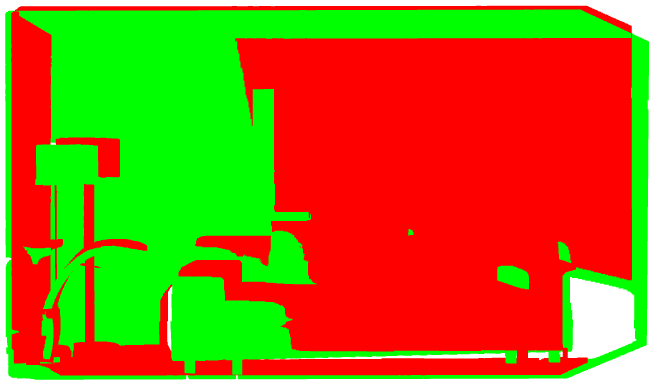
\includegraphics[width=\textwidth]{./results/icp/point_clouds_10_50_before.png}
    \caption{Before}
  \end{subfigure}
  \hfill
  \begin{subfigure}[b]{0.45\textwidth}
    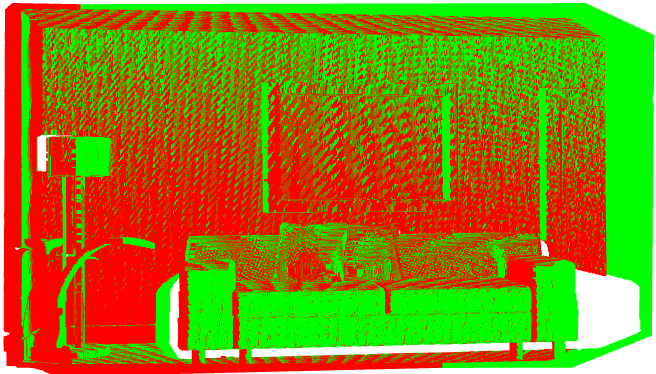
\includegraphics[width=\textwidth]{./results/icp/point_clouds_10_50_after.png}
    \caption{After}
  \end{subfigure}
  \caption{Results with frames 10 and 50}
\end{figure}
\begin{figure}[H]
  \centering
  \begin{subfigure}[b]{0.45\textwidth}
    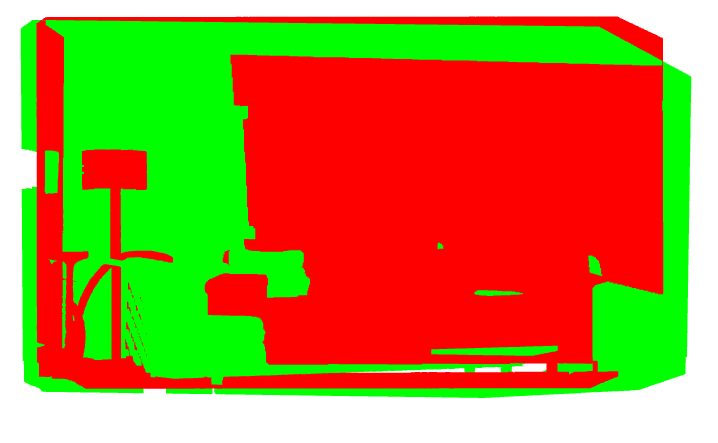
\includegraphics[width=\textwidth]{./results/icp/point_clouds_10_100_before.png}
    \caption{Before}
  \end{subfigure}
  \hfill
  \begin{subfigure}[b]{0.45\textwidth}
    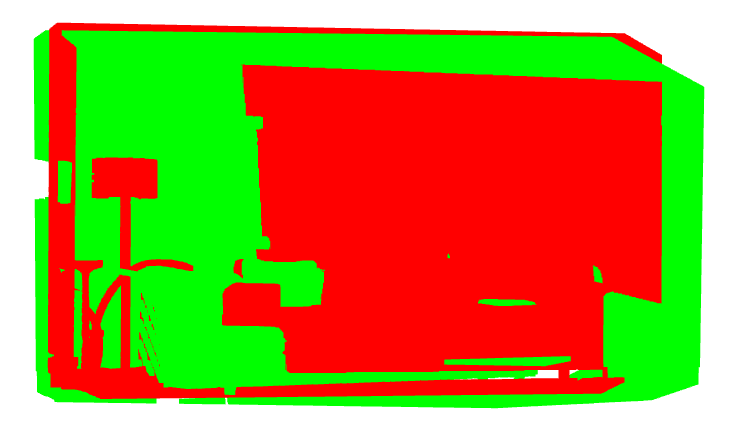
\includegraphics[width=\textwidth]{./results/icp/point_clouds_10_100_after.png}
    \caption{After}
  \end{subfigure}
  \caption{Results with frames 10 and 100}
\end{figure}
The pose estimation fails for frames 10 and 100 because the small pose change assumption is violated.
\section{Point-based Fusion}
\subsection{Merge}
The merge operation for points and normals can be written as
\[p \leftarrow \frac{w\times p + \left(R_c^w\times q + t_c^w\right)}{w+1}\]
\[n_p \leftarrow \frac{w\times n_p + R_c^w\times n_q}{w+1}\]
\[n_p \leftarrow \frac{n_p}{||n_p||_2}\]

\subsection{Results}
\begin{figure}[H]
  \centering
  \begin{subfigure}[b]{0.45\textwidth}
    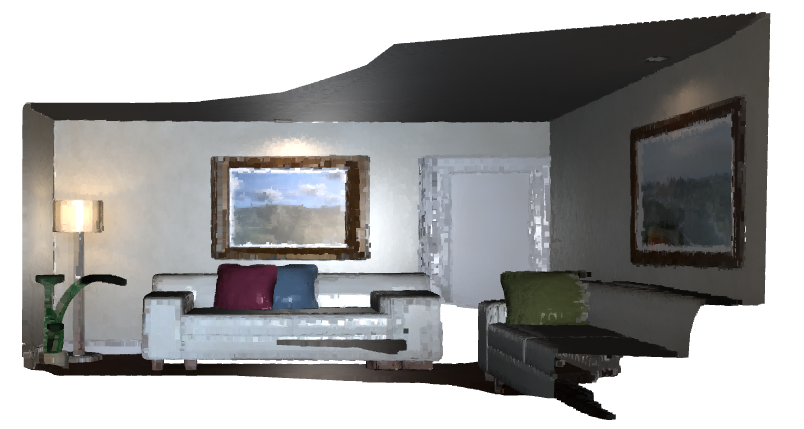
\includegraphics[width=\textwidth]{./results/fusion/rgb.png}
    \caption{RGB}
  \end{subfigure}
  \hfill
  \begin{subfigure}[b]{0.45\textwidth}
    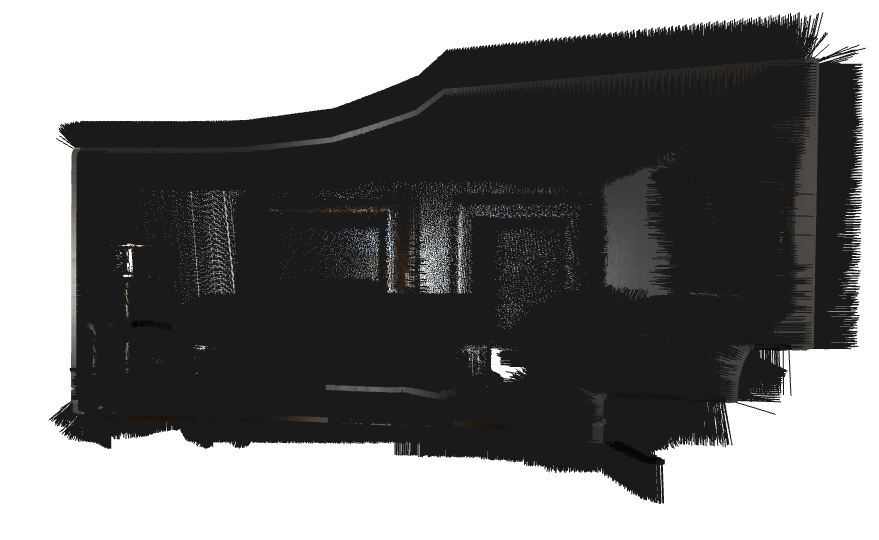
\includegraphics[width=\textwidth]{./results/fusion/normals.png}
    \caption{Normals}
  \end{subfigure}
  \caption{Result of Point-based Fusion}
\end{figure}
Number of points is after fusion is 1362157. The number of points obtained by simple concatenation is 15360000. Therefore, the compression ratio is:
\[\text{Compression Ratio} = \frac{\text{No. of points before fusion}}{\text{No. of points after fusion}} = \frac{15360000}{1362157} = 11.28\]
\section{The dense SLAM system}
\subsection{Source and Target}
The map is the source and the RGBD input is the target.\\\\
One reason why swapping their roles will not work is that in projective data association step of ICP, we first project source points into image plane of target to associate every source point to a target point. Filtering is then performed to remove associations where $(u, v)$ coordinates go out of bounds of target image. These steps are made possible by the fact that target is a regular 2D array of size $H\times W$ and is formed by a camera with known intrinsic parameters. The association and filtering are much harder to perform when target is an unordered point cloud which is the case with the map we store.
\subsection{Results}
\subsubsection{RGB}
\begin{figure}[H]
  \centering
  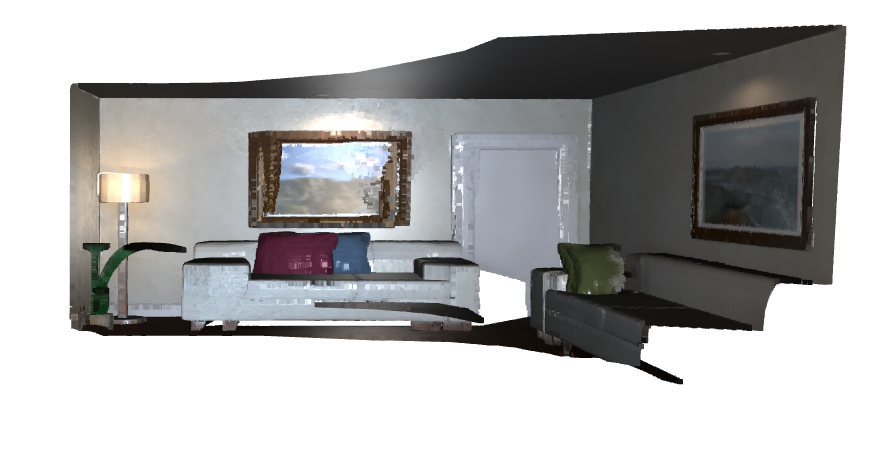
\includegraphics[width=0.8\textwidth]{./results/dense_slam/rgb.png}
  \caption{RGB result}
\end{figure}
\subsubsection{Pose}
\begin{figure}[H]
  \centering
  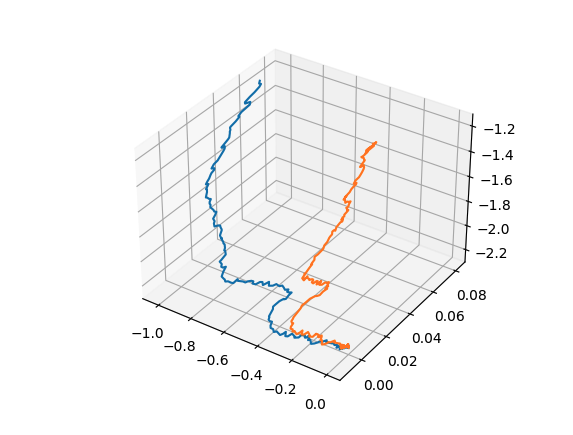
\includegraphics[width=0.8\textwidth]{./results/dense_slam/pose.png}
  \caption{Drift}
\end{figure}
\subsection{[BONUS] Reducing Drift}

\end{document}
